\documentclass{article}
\usepackage{graphicx} % Required for inserting images
\usepackage{tikz}
\usepackage{pgfmath}
\usetikzlibrary{positioning}
\usetikzlibrary{calc}
\usepackage{intcalc}
\usetikzlibrary{shapes.geometric, arrows, positioning}

%%
\begin{document}

\title{TikZ Graph Example}
\author{Ch}
\date{March 19, 2025}

\maketitle

\section{Introduction}
This is an example document to create TikZ graphs.

\section{Annealer Gate Graph}
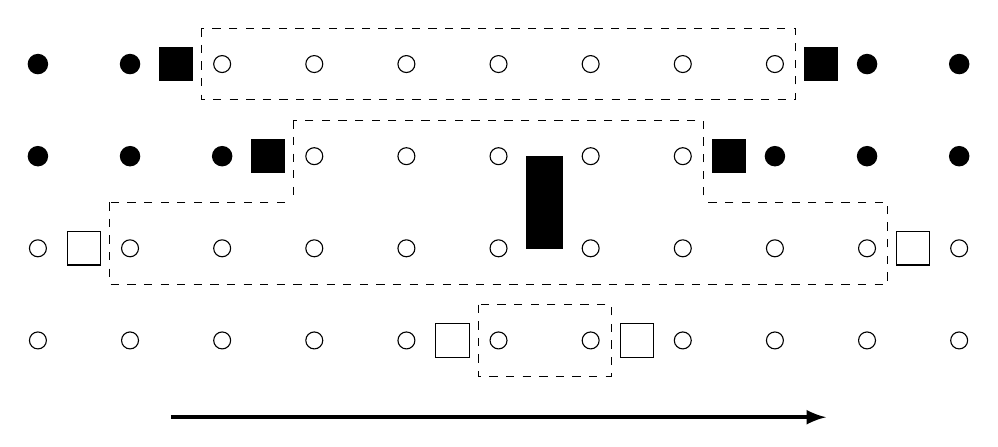
\begin{tikzpicture}[scale=0.65, transform shape]
    % Your TikZ code goes here
    \tikzstyle{round} = [draw=black, circle, minimum size=0.2cm]
    
    % make a round nodes matrix of start at (0, 0) and spaced 1cm using forloop
    \foreach \y in {1, 2, ..., 4} {
        \foreach \x in {1, 2, ..., 11} {
            \node[round] (N\y_\x) at ($(0cm, 0cm) + (\x * 1.8, \y * -1.8)$) {};
        }
    }

    % fill the node I want to fill with black color
    % fill first line with black
    \foreach \x in {1, 2} {
        \fill[black] (N1_\x) circle (0.2cm);
    }
    \foreach \x in {10, 11} {
        \fill[black] (N1_\x) circle (0.2cm);
    }
    % fill second line with black
    \foreach \x in {1, 2, ..., 3} {
        \fill[black] (N2_\x) circle (0.2cm);
    }
    \foreach \x in {9, 10, ..., 11} {
        \fill[black] (N2_\x) circle (0.2cm);
    }
    
    \tikzstyle{box} = [draw=black, rectangle, minimum width=0.65cm, minimum height=0.65cm]
    % draw the Gate between the two nodes using interpolate
    % Black gates
    \node[box, fill=black] (G1_1) at ($(N1_2)!0.5!(N1_3)$) {};
    \node[box, fill=black] (G1_2) at ($(N1_9)!0.5!(N1_10)$) {};
    \node[box, fill=black] (G2_1) at ($(N2_3)!0.5!(N2_4)$) {};
    \node[box, fill=black] (G2_2) at ($(N2_8)!0.5!(N2_9)$) {};
    % White gates
    \node[box, fill=white] (G3_1) at ($(N3_1)!0.5!(N3_2)$) {};
    \node[box, fill=white] (G3_2) at ($(N3_10)!0.5!(N3_11)$) {};
    \node[box, fill=white] (G4_2) at ($(N4_5)!0.5!(N4_6)$) {};
    \node[box, fill=white] (G4_1) at ($(N4_7)!0.5!(N4_8)$) {};

    % create a dashed box around the nodes
    \draw[dashed] ($(N1_3) + (-0.4cm, 0.7cm)$) rectangle ($(N1_9) + (0.4cm, -0.7cm)$);
    \draw[dashed] ($(N4_6) + (-0.4cm, 0.7cm)$) rectangle ($(N4_7) + (0.4cm, -0.7cm)$);
    
    % create a dashed area around the nodes
    \draw[dashed] ($(N2_4) + (-0.4cm, 0.7cm)$) rectangle ($(N2_8) + (0.4cm, -0.9cm)$);
    \draw[dashed] ($(N3_2) + (-0.4cm, 0.9cm)$) rectangle ($(N3_10) + (0.4cm, -0.7cm)$);
    % Clear the overlapped dashed line
    \draw[draw=white, fill=white] ($(N2_4) + (-0.4cm, -0.8cm)$) rectangle ($(N3_8) + (0.4cm, +0.8cm)$);

    \tikzstyle{longbox} = [draw=black, rectangle, minimum width=0.7cm, minimum height=1.8cm]
    % draw the box between four nodes using interpolate
    % Black gates
    \node[longbox, fill=black] (G1_1) at ($(N2_6)!0.5!(N3_7)$) {};
    % Note: the long box gate should be placed after the dashed area, so it will not be overlapped

    % draw the arrow below the nodes to represent the direction of the graph
    \draw[thick, -latex, line width=0.5mm, draw=black] ($(N4_3) + (-1cm, -1.5cm)$) -- ($(N4_9) + (1cm, -1.5cm)$);

\end{tikzpicture}

\section{Annealer Explanation}
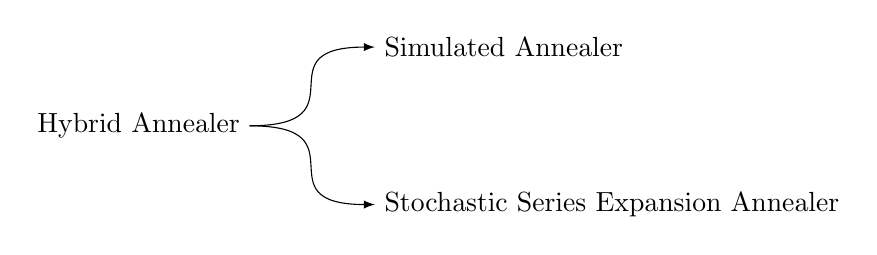
\begin{tikzpicture} [scale=1, transform shape]
    % Make a mind map for Hybrid Annealer to Simulated Annealer and Stochastic Series Expansion Annealer
    \node (HA) [draw, rectangle, draw=white] at (0, 0) {Hybrid Annealer};
    \node (SA) [draw, rectangle, draw=white, anchor=west] at ($(HA) + (3cm, 1cm)$) {Simulated Annealer};
    \node (SSA) [draw, rectangle, draw=white, anchor=west] at ($(HA) + (3cm, -1cm)$) {Stochastic Series Expansion Annealer};

    \draw[-latex] (HA.east) to[out=0, in=180, looseness=2] (SA.west);
    \draw[-latex] (HA.east) to[out=0, in=180, looseness=2] (SSA.west);

\end{tikzpicture}

\section{Maple leaf Graph}
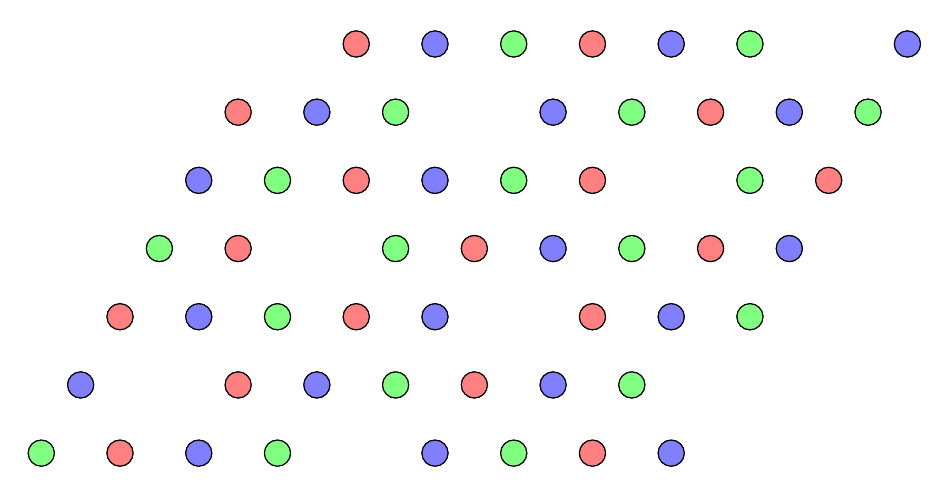
\begin{tikzpicture} [scale=1, transform shape]
    % Make me a Maple leaf nodes graph using forloop and if statement
    \tikzstyle{round} = [draw=black, circle, minimum size=0.2cm]
    
    % make a round nodes matrix of start at (0, 0) and spaced 1cm using forloop
    \foreach \y in {0, 1, ..., 6} {
        \foreach \x in {0, 1, ..., 8} {
            \node (N\y_\x) [
                round, fill=black!50!white
            ] at ($(0cm, 0cm) + (\x*1 + \y*0.5, {\y * sqrt(3) /2})$) {};
        
            % if (x+y+1) mod 3 == 0, then fill the node with blue color
            \pgfmathtruncatemacro{\modval}{mod(2*\x+\y+2, 3)} % Compute (x+y) mod 3
            \ifnum\modval=0
                \node (N\y_\x) [
                    round, fill=blue!50!white
                ] at ($(0cm, 0cm) + (\x*1 + \y*0.5, {\y * sqrt(3) /2})$) {};
            \fi

            % if (x+y+1) mod 3 == 1, then fill the node with red color
            \pgfmathtruncatemacro{\modval}{mod(2*\x+\y+2, 3)} % Compute (x+y) mod 3
            \ifnum\modval=1
                \node (N\y_\x) [
                    round, fill=red!50!white
                ] at ($(0cm, 0cm) + (\x*1 + \y*0.5, {\y * sqrt(3) /2})$) {};
            \fi
            
            % if (x+y+1) mod 3 == 2, then fill the node with green color
            \pgfmathtruncatemacro{\modval}{mod(2*\x+\y+2, 3)} % Compute (x+y) mod 3
            \ifnum\modval=2
                \node (N\y_\x) [
                    round, fill=green!50!white
                ] at ($(0cm, 0cm) + (\x*1 + \y*0.5, {\y * sqrt(3) /2})$) {};
            \fi

            % if y - 3x % 7 == 0, then make the node empty
            \pgfmathtruncatemacro{\modval}{mod(\x + 3*\y +3, 7)} % Compute (y - 3x) mod 7
            \ifnum\modval=0
                \node (N\y_\x) [
                    round, draw=white,
                    fill=white, minimum size=0.4cm
                ] at ($(0cm, 0cm) + (\x*1 + \y*0.5, {\y * sqrt(3) /2})$) {};
            \fi
        }
    }

    
\end{tikzpicture}

\end{document}